\documentclass[10pt]{beamer}

\usetheme{sidebar}
\usepackage[italian]{babel}
\usepackage[utf8x]{inputenc}
\usepackage {eurosym}
\setbeamercovered{transparent}

%
% The following info should normally be given in you main file:
%
\setbeamertemplate{footline}{
\hfill \begin{center}
 \textbf{Pagina \insertframenumber, di \inserttotalframenumber }
\end{center}

}
\title{Revisione dei requisiti}
\author{Team QuiXoft}
\date{12 Dicembre 2008}


\begin{document}
\transduration{1}

\frame{
	\transsplitverticalin
	\titlepage 
\begin{center}
 
\includegraphics[scale=0.20]{logo.png}
\end{center}
}
\part{Analisi dei requisiti}

\frame{
	\transsplitverticalin
	\partpage }

\section{Analisi dei requisiti}
\subsection{Aggiornamento Analisi dei requisiti}
\frame{
	\frametitle{Analisi dei requisiti}
  \framesubtitle{Aggiornamento Analisi dei requisiti}
  
\begin{itemize}
 \item Eliminazione della segreteria generale
 \item Presidente del CCS e Segreteria didattica hanno le stesse funzioni
 \item I docenti verrano invitati tramite mail ad inserire i propri dati
 \item Vincoli dei docenti devono essere motivati, le preferenze no

\end{itemize}
  \transsplitverticalin
	 }

\part{Specifica tecnica}
\frame{
	\transsplitverticalin
	\partpage }
\section{Specifica tecnica}
\subsection{Descrizione dei pattern}
\frame{
  \frametitle{Specifica tecnica}
  \framesubtitle{Descrizione dei pattern}
  \transsplitverticalin
  }
\subsection{Descrizione dei componenti}
\frame{
 \frametitle{Specifica tecnica}
 \framesubtitle{Descrizione dei componenti}
\begin{Large}\textbf{Diagramma dei componenti}\end{Large}
	\begin{center}
 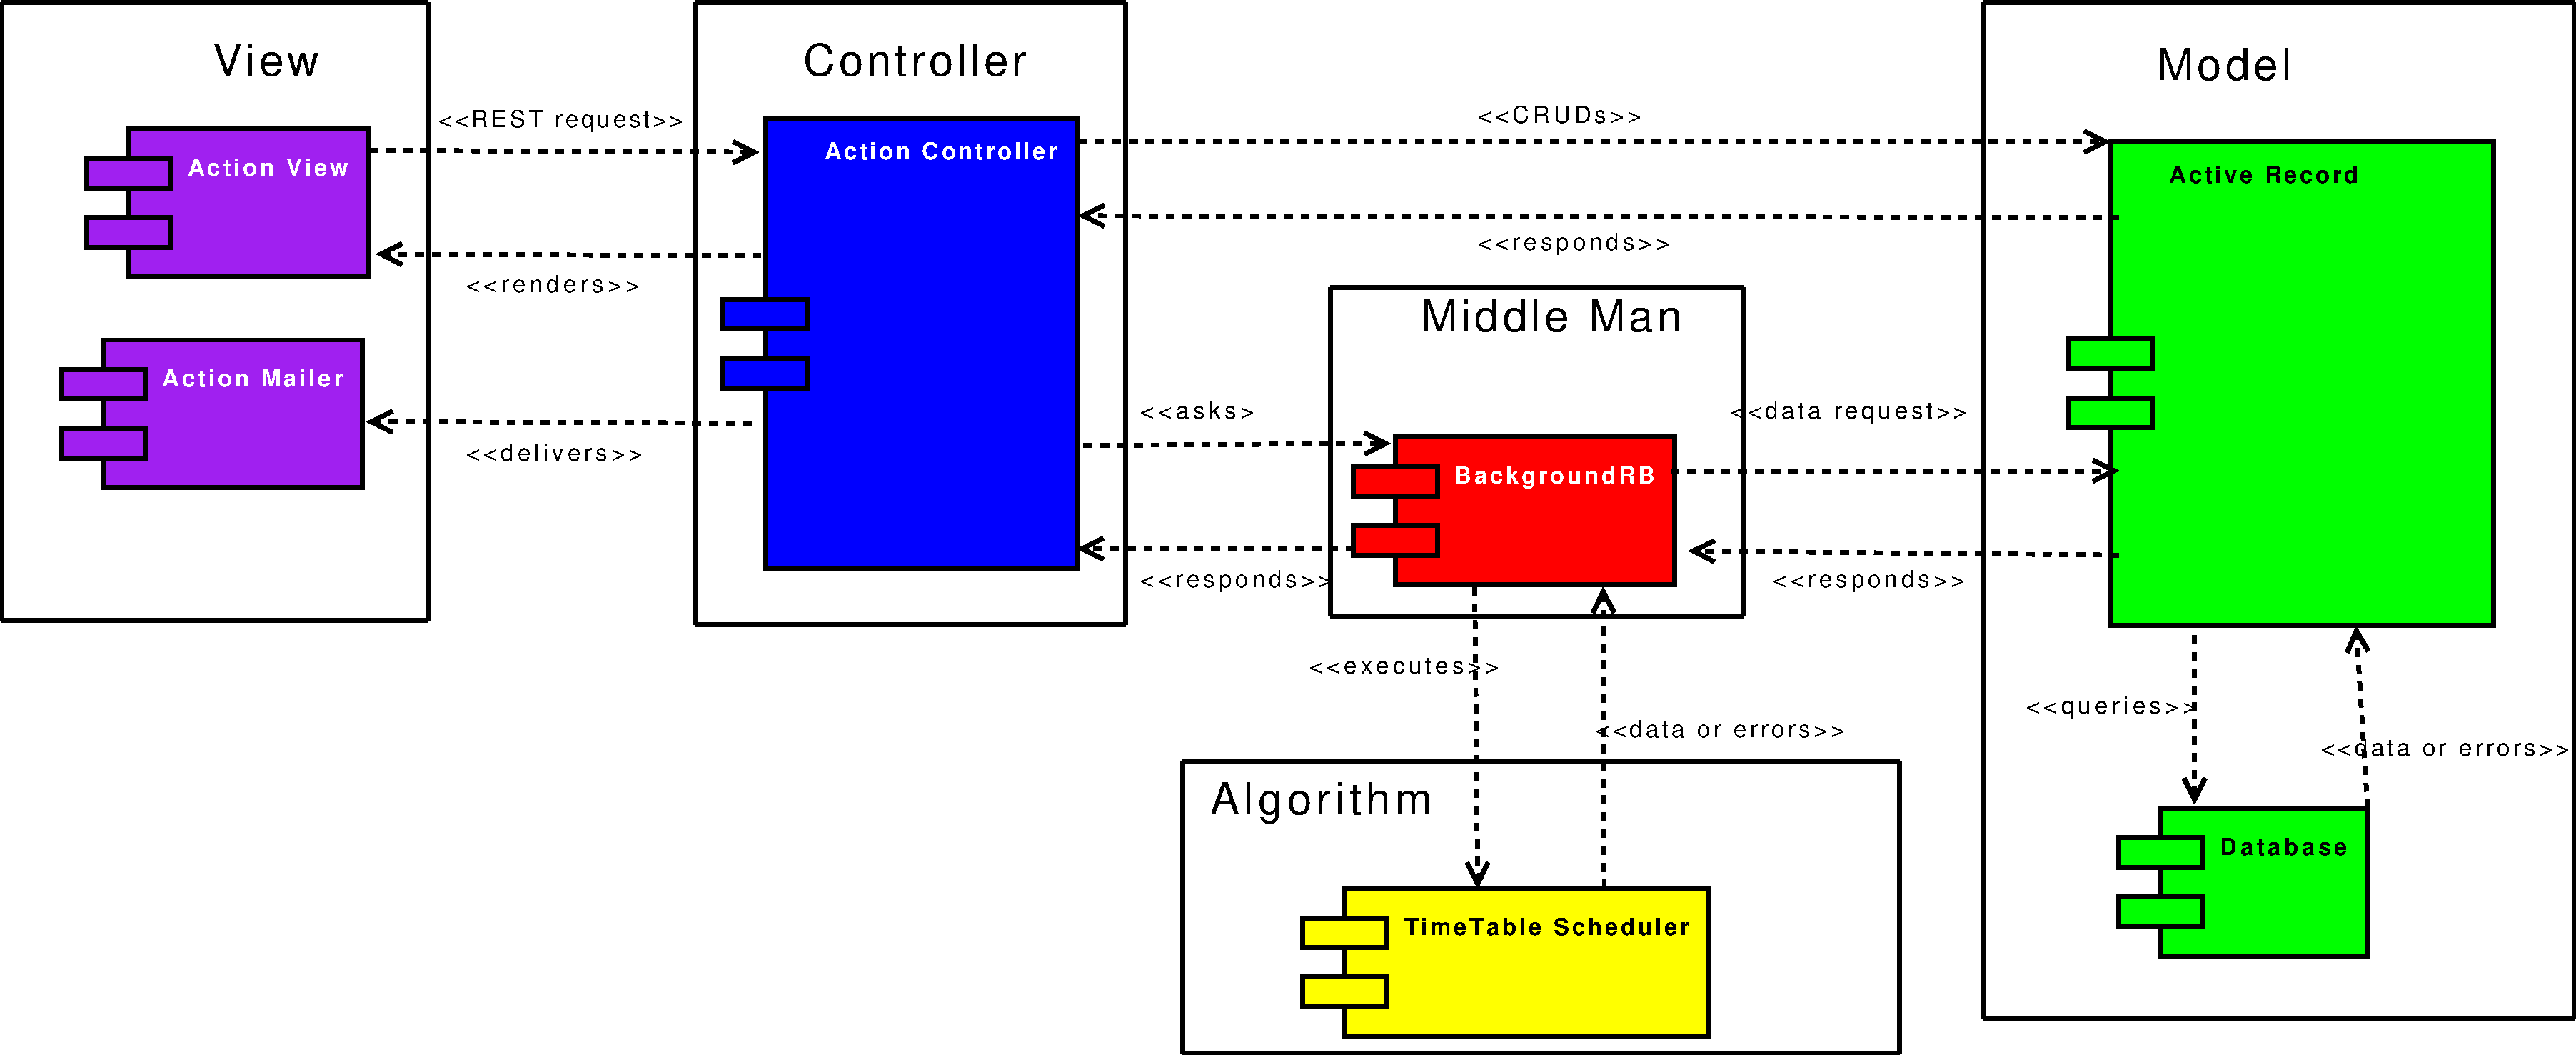
\includegraphics[scale=0.15]{images/diagramma_componenti.pdf}
\end{center}
 \transsplitverticalin
}
\frame{
 \frametitle{Specifica tecnica}
 \framesubtitle{Descrizione dei componenti}
\begin{Large}\textbf{Componente View}\end{Large}
\begin{itemize}
 \item converte le azioni dell'utente in richieste a metodi propri del Controller
\end{itemize}
%Il modulo Action View contenuto nel \underline{framework} \underline{Ruby on Rails}, offre meccanismi avanzati per il riutilizzo del codice, tramite l'uso di viste, \underline{layouts}, partials e di metodi helper pensati per generare ad esempio pagine \underline{XHTML}.
 \transsplitverticalin
}
\frame{
 \frametitle{Specifica tecnica}
 \framesubtitle{Descrizione dei componenti}
\begin{Large}\textbf{Componente Controller}\end{Large}
\begin{itemize}
 \item Action Controller: modulo che gestisce la parte controller;
 \item Ruby on Rails riconosce si serve di un componente chiamato Rounting, per determinare l'azione;
 Es: URL nel formato \textit{controller/azione/id}
\begin{enumerate}
\item viene identificato il Controller \textit{controller}
\item la classe corrispondente viene istanziata
\item l'oggetto richiama il metodo con nome \textit{azione} e con parametro \textit{id}
\item il Controller infine cercherà di visualizzare un \underline{template} con lo stesso nome dell'azione. 
\end{enumerate}	
\item il Controller funge da intermediario fornendo i dati alla View attraverso il Model;
\item sceglie quale view renderizzare a seconda della richiesta pervenuta;
\end{itemize}
 \transsplitverticalin
}\frame{
 \frametitle{Specifica tecnica}
 \framesubtitle{Descrizione dei componenti}
\begin{Large}\textbf{Componente Model}\end{Large}
\begin{itemize}
 \item ActiveRecord: modulo che gestisce la persistenza dei dati;
\item largo uso di convenzioni sui nomi da assegnare a tabelle, classi, colonne e attributi;
\item la classe è descritta dalla tabella che rappresenta ed espone i metodi necessari per leggere e scrivere i record;
\item si relaziona con il Controller ed il Middle Man fornendo i dati che vengono richiesti e salvando le eventuali modifiche al \underline{database}.
\end{itemize}
 \transsplitverticalin
}
\frame{
 \frametitle{Specifica tecnica}
 \framesubtitle{Descrizione dei componenti}
\begin{Large}\textbf{Componente MiddleMan}\end{Large}
\begin{itemize}
 \item componente estranea al pattern MVC;
\item estire quelle richieste che a causa del tempo di calcolo, renderebbero inutilizzabile ogni altra funzione di consultazione dell'applicazione web.
\item implementata tramite un \underline{plugin} per \underline{Ruby on Rails} denominato BackgroundRB
\item soddifare le richieste del Controller preleva, grazie alla sua relazione con il Model, i dati da inviare alla componente Algorithm.
\item informerà il controller lo stesso dell'avanzamento del compito delegatogli, o restituirà i risultati appena disponibili.
\end{itemize}

 \transsplitverticalin
}
\frame{
 \frametitle{Specifica tecnica}
 \framesubtitle{Descrizione dei componenti}
\begin{Large}\textbf{Componente Algorithm}\end{Large}
\begin{itemize}
 \item non inclusa nel \underline{pattern} MVC 
\item calcolare effettivamente l'orario delle lezioni, rispettando i vincoli inseriti nel sistema.
\item restituisce i risultati dei suoi calcoli direttamente alla componente Middle Man.
\end{itemize}
 \transsplitverticalin
}


\subsection{Diagramma delle classi}
\frame{
 \frametitle{Specifica tecnica}
 \framesubtitle{Diagramma delle classi}
 }
\part{Piano di qualifica}
\frame{
	\transsplitverticalin
	\partpage }
\subsection{Aggiornamento piano di qualifica}
\frame{
	\frametitle{Schema generale}
	\transsplitverticalin
	 }\
\end{document}